\chapter{DEM studies}\label{sec:dem-studies}
The discrete element method (DEM) is used by many ceramic breeder researchers to model the interaction of individual pebbles in an ensemble in an effort to obtain a more detailed understanding of pebble beds than is possible with experimental measurements of effective properties. For example see Refs.~\cite{An20071393, Lu2000, Zhao2010, Gan2010a, Annabattula2012a, VanLew2014}.

\subsection{DEM Study: Effective Conductivity with Pebble Damage}
\label{sec:dem-studies-effective-conductivity}
The discrete element method has been used for studies in a variety of fields for studying inter-particle forces and the homogeneously distributed force networks that arise in packed beds (for example, see Ref.~\cite{Makse2000}). The discrete element method was also used in the fusion community to attempt to model crushing initiation and propagation\cite{Annabattula2012a, Zhao2012, Zhao2013}. They too observed that a relatively few number of high-force networks, distributed throughout the bed supported the external mechanical loads. The even distribution of the force networks was used to defend the development of a probability-based predictor for crushing. We make use of the probability argument of Zhao\etal~for the current study\cite{Zhao2013}. Their basic premise is that probability distributions of strength curves for pebble crushing have been observed (see, for example crush loads of Ref.~\cite{Tsuchiya1998}). Then in DEM models, a probability distribution of inter-particle forces are also observed. Overlaying the two probabilities resulted in seemingly random locations of pebbles satisfying the damage criteria -- not strictly along the high-force chains running through packed beds.

We apply the theory of Zhao\etal~in the following manner. If pebbles are crushed in random locations, we may de-couple the task of predicting pebble damage (\textit{i.e.} finding the mechanical or thermal load that causes a pebble to fail) from the task of modeling the ramifications of pebble crushing. Experiments on crushing single, brittle pebbles reveal that there are a number of failure modes\cite{Wu2004}. At one end, the pebble may simply crack and continue to hold a load for some time. At the other extreme, a pebble may crush practically into a dust. We concern ourselves with the latter for this study. When a pebble in our simulation has been flagged for damage, we remove the pebble completely from the ensemble and then allow the remaining pebbles to rearrange to compensate for the lack of equilibrium on their contact forces. 

In our model, we begin with a starting point of a packed bed and then simply flag pebbles at random for crushing. The removal disrupts the meta-static state of the ensemble and the remaining pebbles re-settle due to gravity and the imbalance of contact forces. In reality, the ceramic pebbles generally break into just a few large pieces that remain in the system, a simulation attempting to model such a crush event is covered in \cref{sec:applied-studies}.

\subsubsection{Model Setup \& Methodology}\label{sec:dem-setup}
We analyze a three-dimensional pebble bed consisting of mono-dispersed particles of diameter $d_p$. The particles are constrained by rigid $y-z$-planes at locations of $\frac{x}{d_p} = \pm 10$ (the walls of our container). There are periodic boundary conditions in the $y$-direction located at $\frac{y}{d_p} = \pm 7.5$. Gravity acts in the negative $z$-direction and the particles are resting on a rigid $x-y$-plane at $z=0$ (the floor of the container) and held from the top by an $x-y$-plane at $\frac{z}{d_p} = 30$ (the roof of the container). We pack to $\phi = 64\%$ and, given the volume, have 11000 particles. The volume was chosen to represent the long, tall, narrow channels seen in many solid breeder module designs\cite{ Cho2008, Poitevin2010, Enoeda2003}.

For this study, the material properties were chosen to represent lithium metatinatate pebbles. All the properties come from Ref.~\cite{Gierszewski1998}. They are summarized in Table~\ref{tab:mat-props}

\begin {table}[tp] %
\caption{Maximum load and nominal tension.}
\label {tab:mat-props} \centering %
\begin {tabular}{ cccccc }
\toprule %
E           &     $\nu$    	&    k         	&    C          &   $\alpha$                \\
(GPa)    	&            	& (W/m-K) 		&  (J/kg-K)  	&   (1/K)                   \\\toprule
126			&      0.24     &  2.5          &  1156       	&   $15\times10^{-6}$		\\\bottomrule
\end{tabular}
\end{table}

In the first attempt at packing pebbles into the system, we begin with a common starting point of a filled, lightly packed volume of 10~550 pebbles. We simulate pouring the pebbles into the volume by initializing them into the system from a height of $\frac{z}{d_p} \approx 50$ and allow them to fall under the influence of gravity (see Fig.~\ref{fig:fill01}). We pack the pebbles into a higher packing fraction by means of oscillating the walls as if the pebble bed were sitting on a vibrating plate. This was to imitate the vibration packing technique done in our experimental lab when testing pebble beds in the uniaxial compression test stand. The vibration scheme was able to slowly densify the packed bed but, owing to the very small timestep of the simulation, the simulation times were impractically large to approach a packing fraction greater than $\phi = 60\%$. 

\begin{figure}[!ht]
	\centering
	\begin{subfigure}[b]{0.25\textwidth}
		\centering
		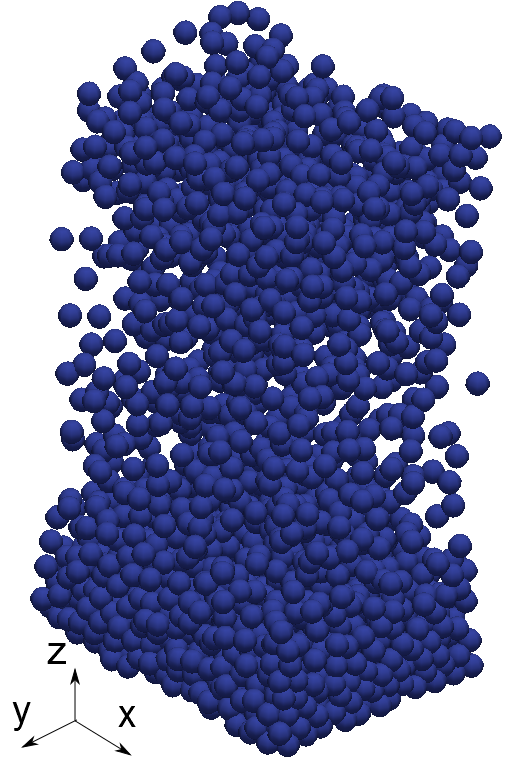
\includegraphics[width=\textwidth]{chapters/figures/fill01.png}
	\end{subfigure}
	\begin{subfigure}[b]{0.25\textwidth}
		\centering
		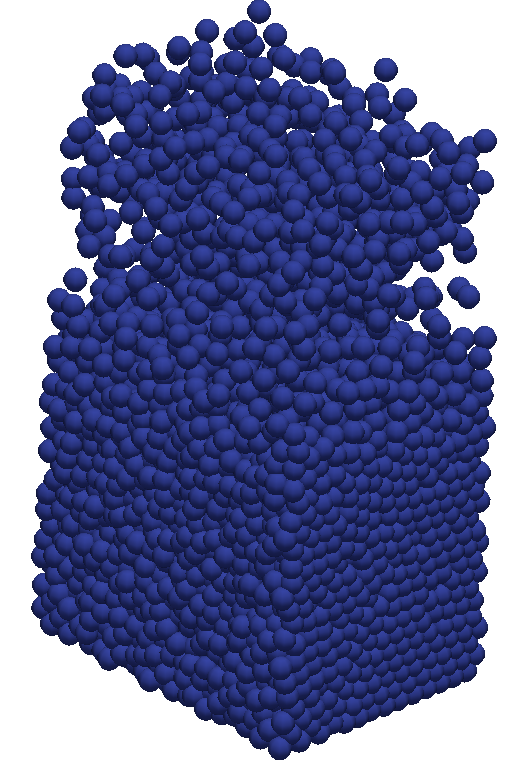
\includegraphics[width=\textwidth]{chapters/figures/fill02.png}
	\end{subfigure}
	\begin{subfigure}[b]{0.25\textwidth}
		\centering
		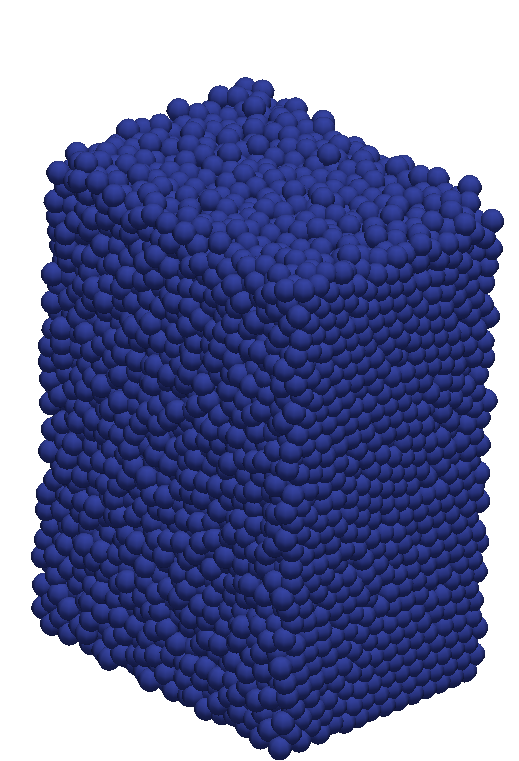
\includegraphics[width=\textwidth]{chapters/figures/fill03.png}
	\end{subfigure}
	\caption{Demonstrating the pouring process of $N = 10550$ pebbles into the control volume with at an early time (left), when it is nearly filled (middle) and after the pebbles have settled to negligible kinetic energy (right).}
\label{fig:fill01}
\end{figure}

In the end, a simpler pack-relax method was used instead. In this method $N$ particles are inserted into the volume such that we have precisely the packing fraction we desire (in this case, $\phi = 64\%$ so $N = 11000$). The pebbles are placed at random into the volume and are allowed to artificially overlap -- often by a great deal ($\delta \sim R_p$). The overlap they experience would normally cause such an enormous force (integrating into an enormous velocity) that the pebbles would all explode out of the bed at the first step in time integration. We avoid such a catostrophic scenario with a relaxation scheme where we truncate the displacement of any pebble per timestep that is integrated from the force. The truncated displacement is very small and allows the pebbles to slowly move away from each other and into a static equilibirum as the artifical overlap is reduced. Once the pebble bed comes to rest, we remove the relaxation (limiting displacement command) and allow standard integration of contact forces with the velocity-Verlet algorithm (see \cref{sec:velocity-verlet}). The pack-relax scheme allowed for obtaining desireable, highly repeatable packing fractions for all pebble beds. Once the pebble bed was packed into an initial condition, the simulation state was saved and used as a starting point for the numerous `crushed' cases to be described later.

In this first study, we model pebble crushing without considering why the particular pebble should be cracking. In the model we randomly select pebbles from the ensemble, regardless of forces acting upon the pebble, and delete them entirely from the system. When a pebble is removed, the neighboring pebbles react due to the imbalance of forces, and the bed settles into a new configuration. We differentiated the failed beds by their percentage of failed pebbles: $\eta = $ number of failed pebbles per original ensemble size. For the baseline case and for beds after failing, we apply the heating routine described next.

To simulate the conditions of a solid breeder in a fusion reactor, where the heat is removed from the pebble bed via contact to the containing structure, we assigned a constant temperature of $T_\text{c}$ to the vertical walls. Nuclear heating of the pebbles is simulated through a constant source term on each pebble. A representative heating rate of $Q_s = q_p'''V_p$, where  $q_p'''= 8$ MW/m$^3$. The heating cycle runs until a thermal steady state is reached. Based on a measurement of the total thermal energy of the bed, $E_T =\sum_i^N m_iC_i T_i$, steady-state is determined as $\dt{E_T} = 0$ within a specified tolerance. Once at steady state, we analyzed thermal and mechanical characteristics of the pebble bed: effective thermal conductivity, average coordination number, temperature profiles in the bed, and inter-particle contact forces. 

Based on the boundary conditions to our system, we establish heat transfer that is symmetric and one-dimensional in the $x$-direction from $x=0$ to the walls at $\frac{x}{d_p} = \pm 10$. As we will show, the pebble bed has very little variation of forces and temperatures in the $y$-direction due to the periodic boundary condition at the edges of the domain. Gravity effects are minor in the overall heat transfer and induce only a slight $z$-dependency to the results. We take advantage of this nature of our pebble bed to find the effective conductivity from an analytic, one-dimensional test case.
%~~~~~~~~~~~~~~~~~~~~~~~~~~~~~~~~~~~~~~~~~~~~~~~~~~~~~~~~~~~~~~~~~~~~~~





%~~~~~~~~~~~~~~~~~~~~~~~~~~~~~~~~~~~~~~~~~~~~~~~~~~~~~~~~~~~~~~~~~~~~~~
\subsubsection{Effective Thermal Conductivity from Analytic Analogy}
Assuming a one-dimensional pebble bed, to find an effective conductivity, we step back into a continuum mechanics formulation where the pebble bed can be represented as a slab of solid material. We can analytically solve for the temperature equation in a slab with heat generation, symmetry about the centerline, and a constant boundary temperature condition.

At steady-state, the temperature of a material with constant temperature boundary conditions ($T(L) = T_s$), constant thermal conductivity ($k_\text{eff}$), and nuclear heating ($q'''$) obeys the following equation

\begin{equation}\label{eq:continuum-heateqn}
	0 = \frac{\mathrm{d}^2T}{\mathrm{d}x^2} + \frac{q'''}{k_\text{eff}}
\end{equation}

We introduce a non-dimensional temperature
\begin{equation}
	\theta = \frac{T(x) - T_s}{T_0 - T_s}
\end{equation}
where $T_0$ is the temperature at the centerline of this slab (a value we will find momentarily). The length is non-dimensionalized as
\begin{equation}
	x^* = \frac{x}{L}
\end{equation}

Thus we can re-write Eq.~\ref{eq:continuum-heateqn} as
\begin{equation}\label{eq:continuum-heateqn-nondim}
	0 = \frac{\mathrm{d}^2\theta}{\mathrm{d}x^{*2}} + G
\end{equation}
where
\begin{equation}
	G = \frac{q'''L^2}{k_\text{eff}(T_0 - T_s)}
\end{equation}

In the non-dimensionalized form, the solution is revealed to be purely geometric,
\begin{equation}\label{eq:continuum-temperature-nondim}
	\theta = 1-x^{*2}
\end{equation}. 
as $T_0  - T_s = \frac{q'''L^2}{2k_\text{eff}}$. We will use the non-dimensional temperature solution of Eq.~\ref{eq:continuum-temperature-nondim} to prove our one-dimensional assumption of heat transfer is justified for the pebble beds.

We note that in this continuum mechanics formulation, we are assuming that the nuclear source, $q'''$ term is applied evenly over the entire volume. In our DEM formulation, our source term applies to a single pebble. To find the effective thermal conductivity of our `slab' of pebble bed, we must reconcile this discrepency. This is accomplished with the exchange of
\begin{equation}\label{eq:q-source-translation}
	q''' = \frac{Q_\text{tot}}{V_\text{tot}} = \frac{Q_sN}{H\cdot L\cdot W\cdot d_p^2}
\end{equation}
where the pebble bed volume is given by the height, $H$, width, $W$, and length, $L$, and $Q_s$ is the source term on each pebble in the DEM ensemble. 

From the solution of Eq.~\ref{eq:continuum-heateqn-nondim}, we find the effective conductivity to be
\begin{equation}
	k_\text{eff} = \frac{q''' L^2}{2(T_0-T_s)}
\end{equation}
and when we replace the heat generation term with Eq.~\ref{eq:q-source-translation}, and use the bed dimensions as given in \cref{sec:dem-setup}, this is written as
\begin{equation}\label{eq:dem-effecitve-conductivity-formula}
	k_\text{eff} = \frac{Q_sN}{180(T_0-T_s)d_p}
\end{equation}

We will use this formulation of Eq.~\ref{eq:dem-effecitve-conductivity-formula} to analyze and compare the pebble beds of this study.
% \begin{figure}[htbp]
% 	\centering
% 	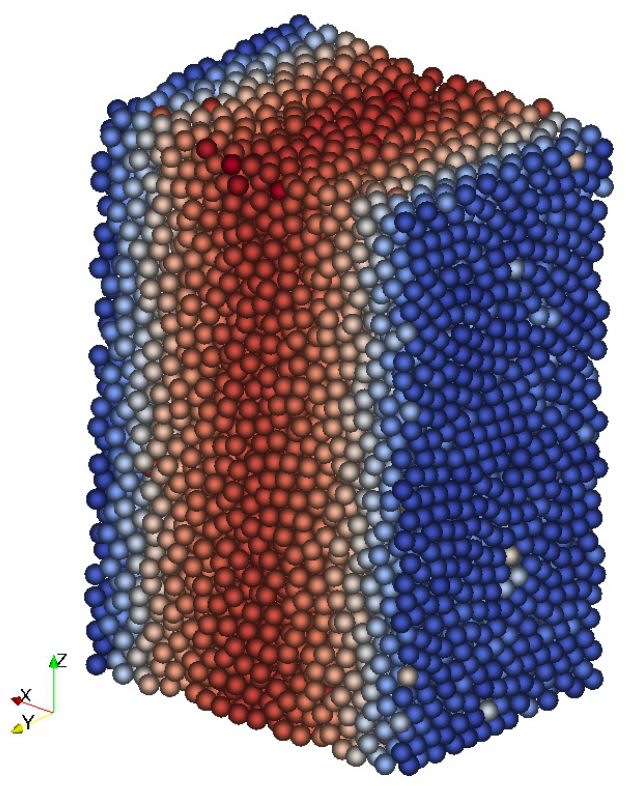
\includegraphics[trim=1cm 8cm 3cm 4cm, width=0.5\textwidth]{chapters/figures/pebbleBedTemperature}
% 	\caption{Temperature distribution of pebbles in the $10\%$ failed bed. At the end of steady-state heating, a one-dimensional profile is evident in all pebble beds studied here. The pebbles are receiving nuclear heating. Cooling proceeds through the pebbles in contact with the walls in the $x$-direction.}
% \label{fig:pebbleBedTemperature}
% \end{figure}



\subsubsection{Results}
The aim of this study was both to discover the impact of pebble failure on thermo-mechanical properties as well as determine the impact as a function of the number of failed pebbles. To satisfy the latter, we created beds with $\eta = 1\%$, $3\%$, $5\%$, $10\%$, and $15\%$ of pebbles failed. 

We plot Eq.~\ref{eq:continuum-temperature-nondim} against the non-dimensionalized temperature profiles coming from the steady-state DEM simulation in Fig.~\ref{fig:temp-scatters}. We find that all our models had a nearly perfect match to a one-dimensional prediction, validating the calculation of effective thermal conductivity in this study. Furthmore, the profiles adhering to the one-dimensional curve also allows us to find the effective conductivity of each bed from applying Eq.~\ref{eq:dem-effecitve-conductivity-formula}, which was derived from the one-dimensional assumption.

One concern we had for pebble crushing, was the phenomenon of `jamming' during resettling that would possibly leave pebbles isolated from their neighbors (apart from those they are resting upon). Jamming can happen when a bridge of pebbles have a balance for forces without strong or any contact to a pebble below them. The pebble under the bridge then only has light contact with the pebbles upon which it is resting. Such an isolated pebble would have no strong pathway for heat transfer and heat up much higher than that of its neighbors. Evidence of pebble isolation is apparent in hot individual pebbles above the grouped curve in Fig.~\ref{fig:temp-scatters}. 

\begin{figure}[htbp]
	\centering
	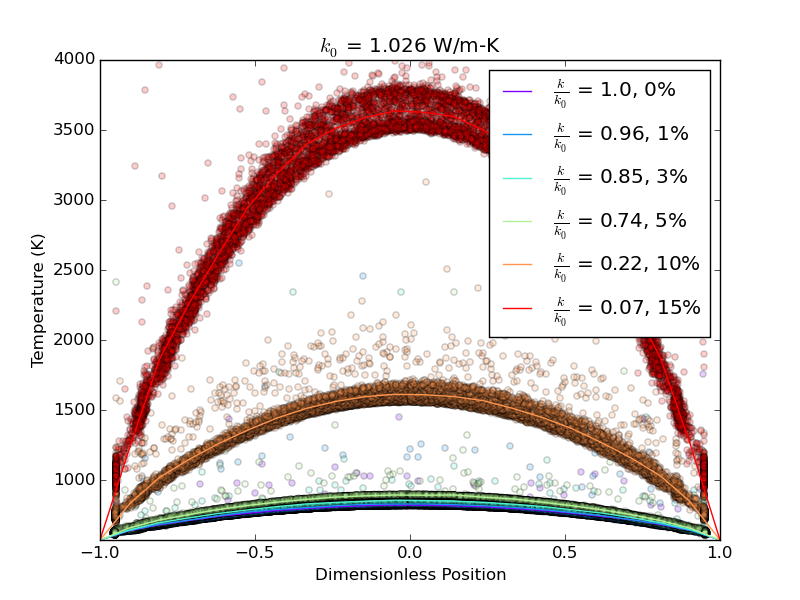
\includegraphics[width=0.65\textwidth]{chapters/figures/dem-evap-0-15-scatter-keff.png}
	\caption{The nondimensional temperature profiles for each test case follow the theoretical shape of a one-dimensional, constant $k$, continuum solution.}
\label{fig:temp-scatters}
\end{figure}

Because the 10\% and 15\% cases have such high temperatures, we show only the 0-5\% crushed together in Fig.~\ref{fig:temp-scatters-zoomed}

\begin{figure}[htbp]
	\centering
	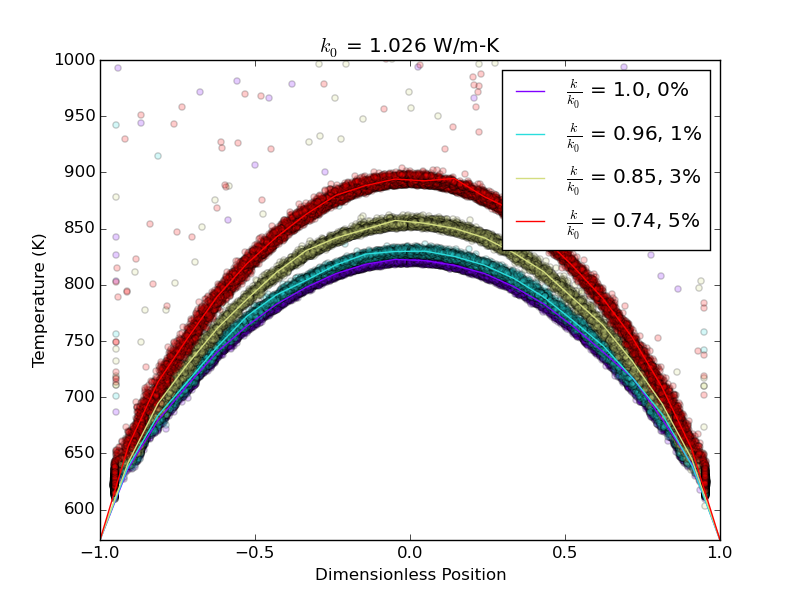
\includegraphics[width=0.65\textwidth]{chapters/figures/dem-evap-0-5-scatter-keff.png}
	\caption{The nondimensional temperature profiles for the test cases up to 5\% crushed pebbles.}
\label{fig:temp-scatters-zoomed}
\end{figure}

The individual hot pebbles in Fig.~\ref{fig:temp-scatters} are also indicative of the shortcomings of the discrete element method for modeling solid breeders in fusion reactors. The flowing purge gas in actual solid breeders would likely not permit such thermal isolation of pebbles. Even if a pebble had no physical contact with neighboring ones, it would still transport energy via conduction and advection of the helium gas. This will be addressed again and in more detail in \cref{sec:cfd-dem-effective-conductivity}.

In order to calculate an effective conductivity of the pebble bed, we must find an average temperature profile through the bed to compare with Eq.~\ref{eq:continuum-temperature-nondim} and thus employ Eq.~\ref{eq:dem-effecitve-conductivity-formula}. We compare steady-state temperature profiles in the test beds against the one-dimensional, non-dimensional temperature profile. Average values of the bed, along the $x$ direction, are generated via averaging temperatures in bins. We create bins that are volumes slices of width $\Delta x$ that extend through the limits of the $y$- and $z$-directions. We then find the $n$ pebbles residing in the slices and take the mean value of their temperatures. The average, given by Eq.~\ref{eq:binned-T}, is also given in Fig.~\ref{fig:temp-scatters}. The binned average temperature is 
\begin{equation}\label{eq:binned-T}
	\langle T\rangle = \frac{1}{n}\sum_{i}^n T_i 	
\end{equation}
Using the volume slices, we also find the average coordination number, 
\begin{equation}\label{eq:binned-z}
	\langle Z \rangle = \frac{1}{n}\sum_{i}^n Z_i
\end{equation}
and average contact force, 
\begin{equation}\label{eq:binned-f}
	\langle F^{1/3} \rangle = \frac{1}{n}\sum_{i}^n F_{n,ij}^{1/3}
\end{equation}


In Eq.~\ref{eq:thermoFirstLaw} of \cref{sec:dem-heat-transfer}, we see that at steady-state, the energy input by nuclear heating must be balanced by the transport of heat out of a pebble into its neighbors. Inter-particle heat transfer is dictated by the number of neighboring contacts, temperature difference between pebbles, and the thermal conductance, $H_{c}$, through the contact area. The thermal conductance (see Eq.~\ref{eq:dem-conductance}) is itself a function purely of material properties  (which are essentially constant here) and the force at the contact, going as $H_{c} \propto F_{n,ij}^{1/3}$. Thus, we write the net heat out of a pebble at steady state as a function of the three variables,

\begin{equation}
	Q_\text{net} =f( Z, F_n^{1/3}, \Delta T)
\end{equation}

The coordination number and contact forces are features of the packing structure in the packed bed that we can analyze to discover what happens to the heat flux between pebbles when the bed experiences crushed particles. Conversely, the $\Delta T$ between two pebbles is the effect of the thermal transport (i.e. leading to higher bed temperatures such as those of Fig.~\ref{fig:temp-scatters}). We will first analyze the changes to the coordination numbers of pebbles in the ensemble as pebbles crush.


\begin{figure}[!ht]
	\centering
	\begin{subfigure}[b]{\doubleimagewidth}
		\centering
		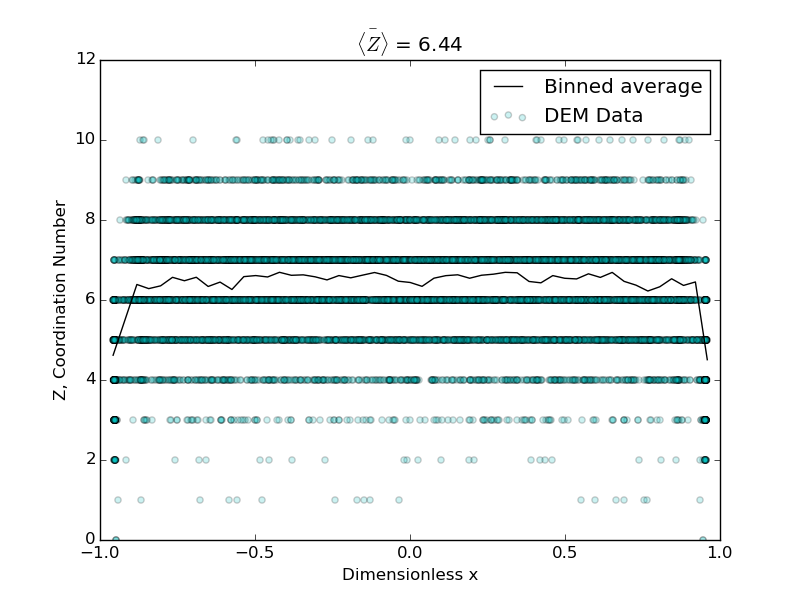
\includegraphics[width=\textwidth]{chapters/figures/heating_dte-02/dem-evap-0-scatter-coord.png}
		\caption{Baseline pebble bed (0\% crushed)}
	\end{subfigure}
	\begin{subfigure}[b]{\doubleimagewidth}
		\centering
		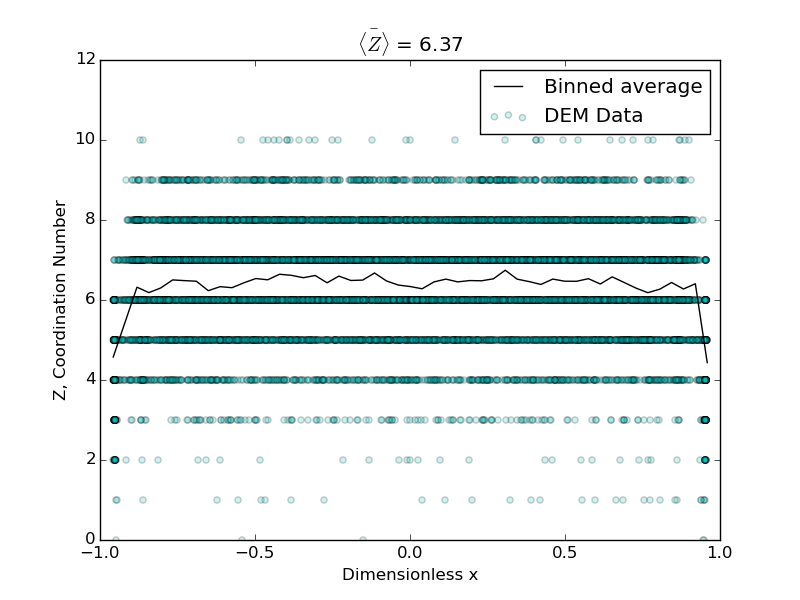
\includegraphics[width=\textwidth]{chapters/figures/heating_dte-02/dem-evap-1-scatter-coord.png}
		\caption{1\% crushed}
	\end{subfigure}
	
	\begin{subfigure}[b]{\doubleimagewidth}
		\centering
		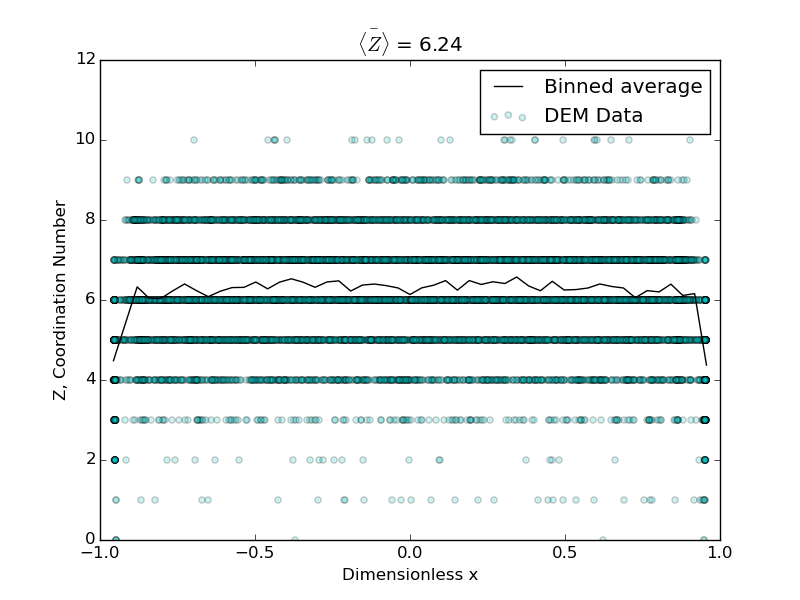
\includegraphics[width=\textwidth]{chapters/figures/heating_dte-02/dem-evap-2-scatter-coord.png}
		\caption{3\% crushed}
	\end{subfigure}
	\begin{subfigure}[b]{\doubleimagewidth}
		\centering
		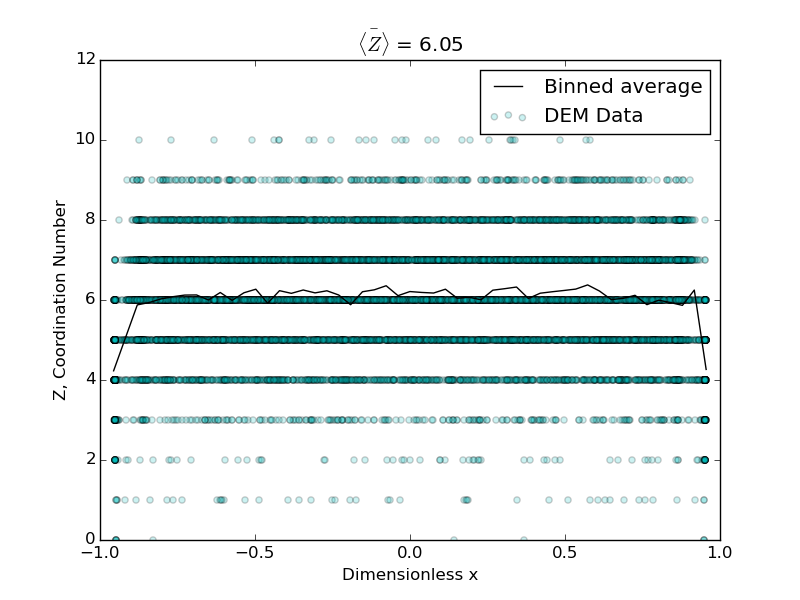
\includegraphics[width=\textwidth]{chapters/figures/heating_dte-02/dem-evap-3-scatter-coord.png}
		\caption{5\% crushed}
	\end{subfigure}

	\begin{subfigure}[b]{\doubleimagewidth}
		\centering
		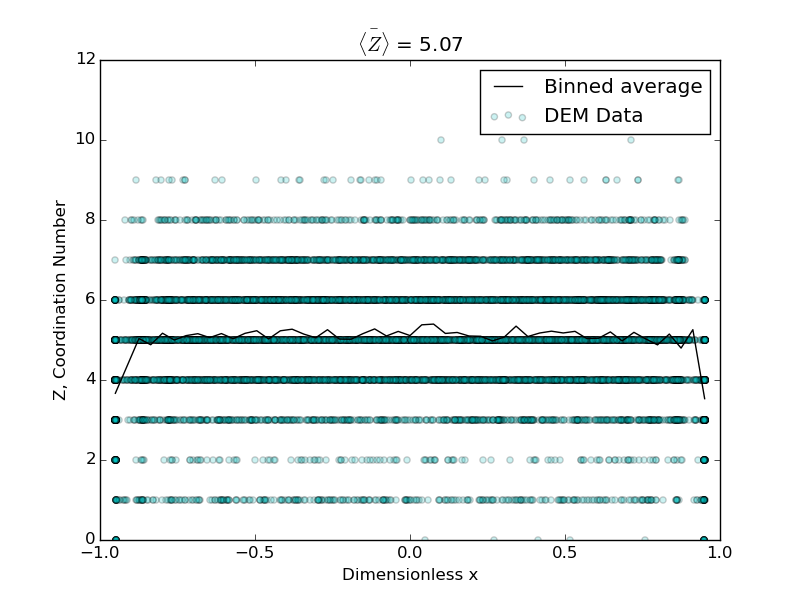
\includegraphics[width=\textwidth]{chapters/figures/heating_dte-02/dem-evap-4-scatter-coord.png}
		\caption{10\% crushed}
	\end{subfigure}
	\begin{subfigure}[b]{\doubleimagewidth}
		\centering
		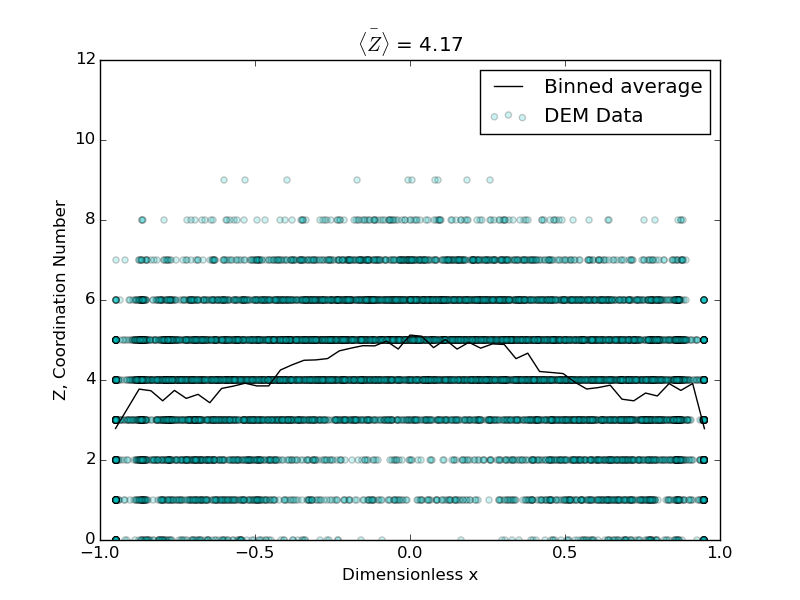
\includegraphics[width=\textwidth]{chapters/figures/heating_dte-02/dem-evap-5-scatter-coord.png}
		\caption{15\% crushed}\label{fig:coord-scatter-15percent}
	\end{subfigure}
	\caption{The average coordination number decreases slowly as the number of broken pebbles in the ensemble increases.}
\label{fig:coord-scatter}
\end{figure}

In Fig.~\ref{fig:coord-scatter} we plot the data for all pebbles in the ensemble as well as the binned average (Eq.~\ref{eq:binned-z}). Clearly, there are fewer average contacts per pebble in the ensemble after failure; At 15\% crushed the coordination number drops by roughly 30\%. But this alone can not not account for the reduction in $k_\text{eff}$ by 93\% for the same amount of crushed pebbles. Next we look to the normal contact forces between pebbles in the bed.


\begin{figure}[!ht]
	\centering
	\begin{subfigure}[b]{0.4\textwidth}
		\centering
		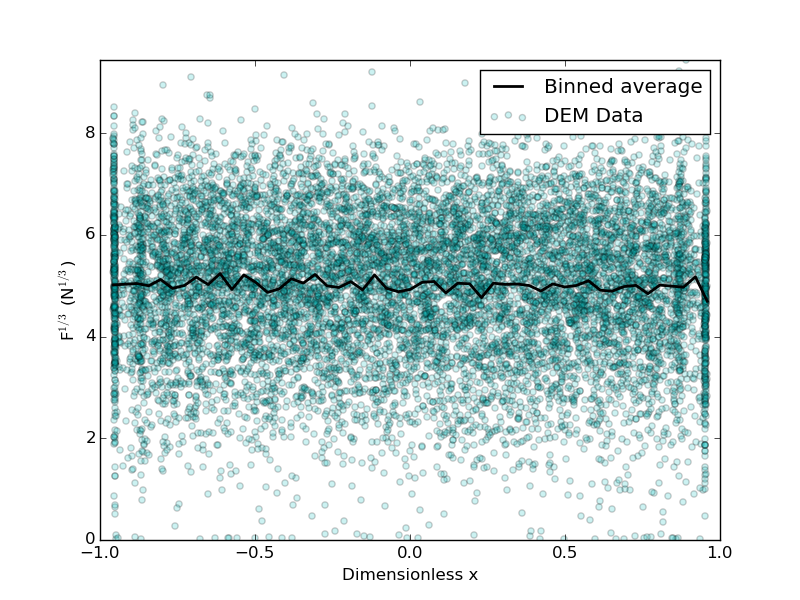
\includegraphics[width=\textwidth]{chapters/figures/heating_dte-02/0/dump/force-profile.png}
		\caption{Baseline pebble bed (0\% crushed)}
	\end{subfigure}
	\begin{subfigure}[b]{0.4\textwidth}
		\centering
		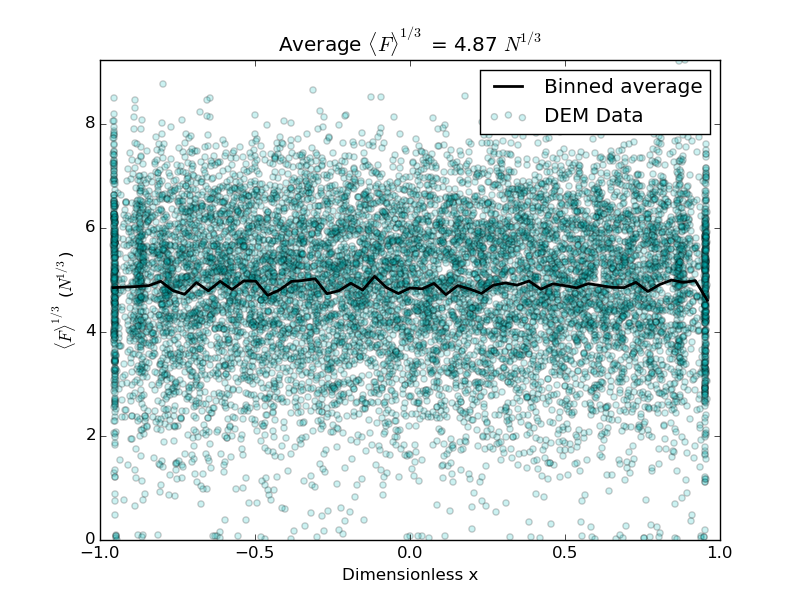
\includegraphics[width=\textwidth]{chapters/figures/heating_dte-02/1/dump/force-profile.png}
		\caption{1\% crushed}
	\end{subfigure}
	
	\begin{subfigure}[b]{0.4\textwidth}
		\centering
		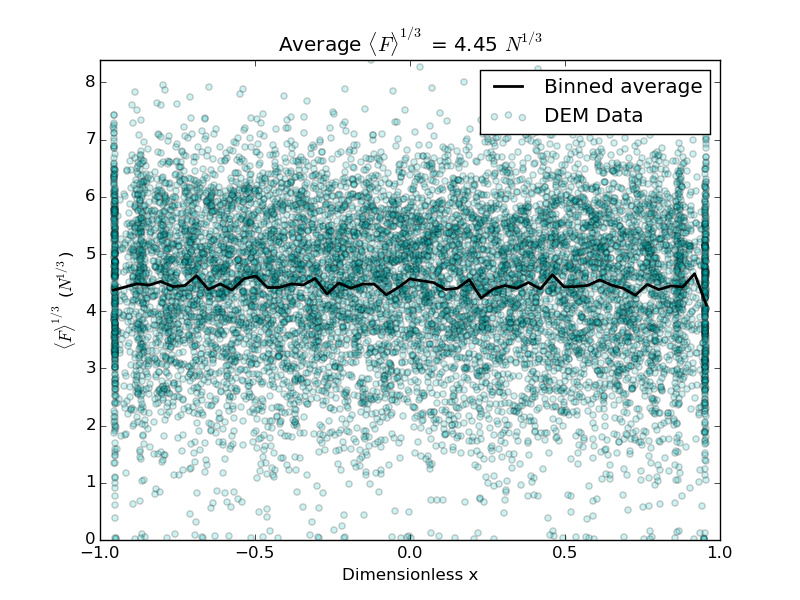
\includegraphics[width=\textwidth]{chapters/figures/heating_dte-02/3/dump/force-profile.png}
		\caption{3\% crushed}
	\end{subfigure}
	\begin{subfigure}[b]{0.4\textwidth}
		\centering
		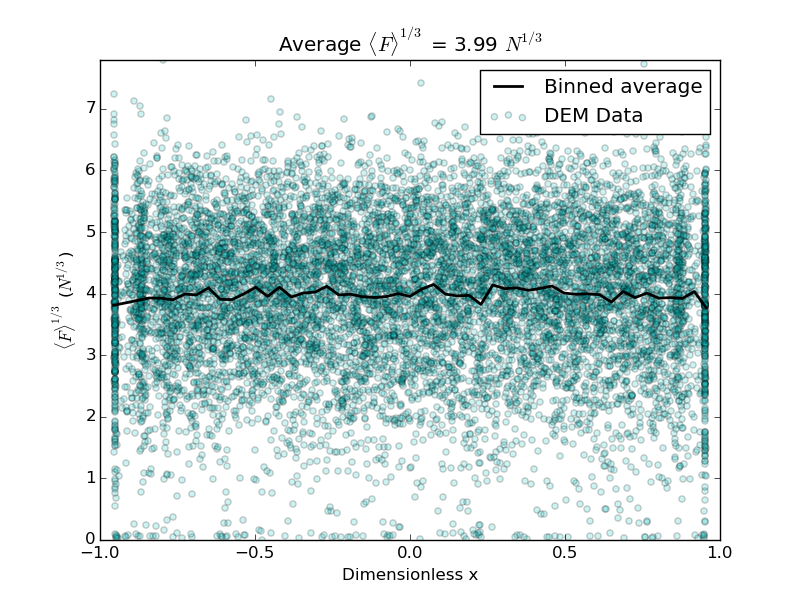
\includegraphics[width=\textwidth]{chapters/figures/heating_dte-02/5/dump/force-profile.png}
		\caption{5\% crushed}
	\end{subfigure}

	\begin{subfigure}[b]{0.4\textwidth}
		\centering
		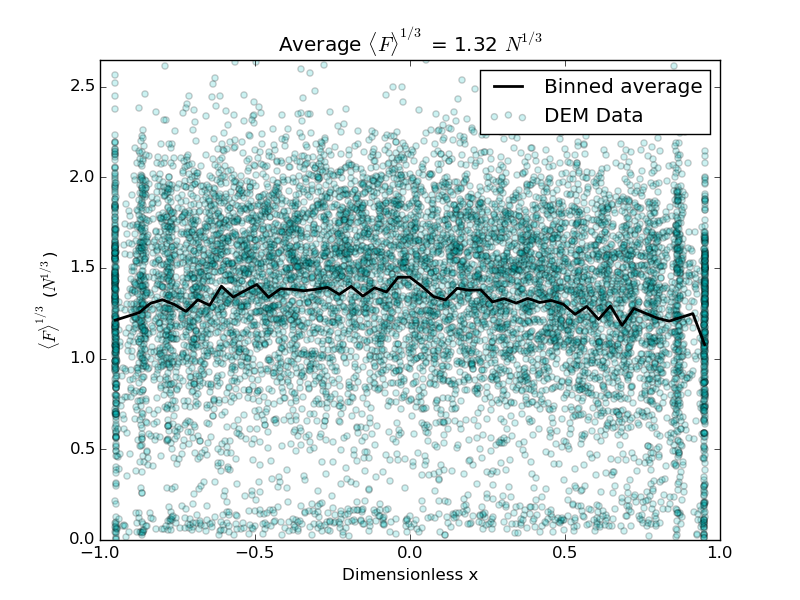
\includegraphics[width=\textwidth]{chapters/figures/heating_dte-02/10/dump/force-profile.png}
		\caption{10\% crushed}
	\end{subfigure}
	\begin{subfigure}[b]{0.4\textwidth}
		\centering
		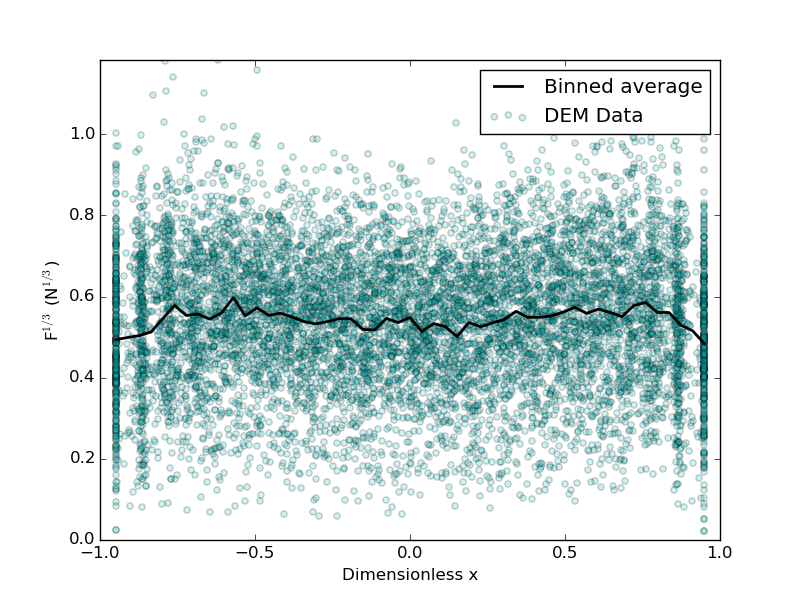
\includegraphics[width=\textwidth]{chapters/figures/heating_dte-02/15/dump/force-profile.png}
		\caption{15\% crushed}\label{fig:contact-forces-scatter-15percent}
	\end{subfigure}
	\caption{As pebble beds experience massive amounts of crushed pebbles (>5\%), the contact forces in the ensemble (after heating to steady-state) show dramatic reductions in value. Note the change of scale on the figures from the baseline case to the 15\% crushed case.}
\label{fig:contact-forces-scatter}
\end{figure}

The normal contact forces between pebbles are plotted in Fig.~\ref{fig:contact-forces-scatter}. A dramatic reduction in the normal forces is seen after many of their neighbors are crushed and are removed from the system. From the baseline down to the 15\% failed case, the contact forces are reduced by about a factor of 10 - similar to the reduction in effective conductivity.

The effective thermal conductivity was found for all of our pebble beds, via Eq.~\ref{eq:dem-effecitve-conductivity-formula}, then normalized against the conductivity of the baseline ensemble ($k^* = k/k_\text{0}$). The average coordination number of the beds and average normal contact forces were also found. Another way of describing a pebble bed is with the packing fraction, $\phi$. In Fig.~\ref{fig:packing-fraction}, we collect all these values (and normalize them against the baseline case) to provide a direct comparison to their changes as a function of crushed pebbles. When $15\%$ of the pebbles are crushed in a pebble bed, the effective conductivity has fallen all the way to only $k^*=0.07$. This large reduction is especially important in light of the already poor thermal management of virgin pebble beds that, even in helium environments, have been experimentally measured at only approximately 1~W/m-K (see, { e.g.}, Refs.~\cite{Reimann:2002mi, Piazza2002811}). The only parameter to have similar reductions in value is the average normal contact force, a value which is seen to follow closely to the curve of effective conductivity. Thus we conclude that the single most important factor for determining the effective thermal conductivity in these pebble beds is the normal contact forces between pebbles; a force which decreases sharply as pebbles are crushed in the system.

\begin{figure}[!ht]
	\centering
	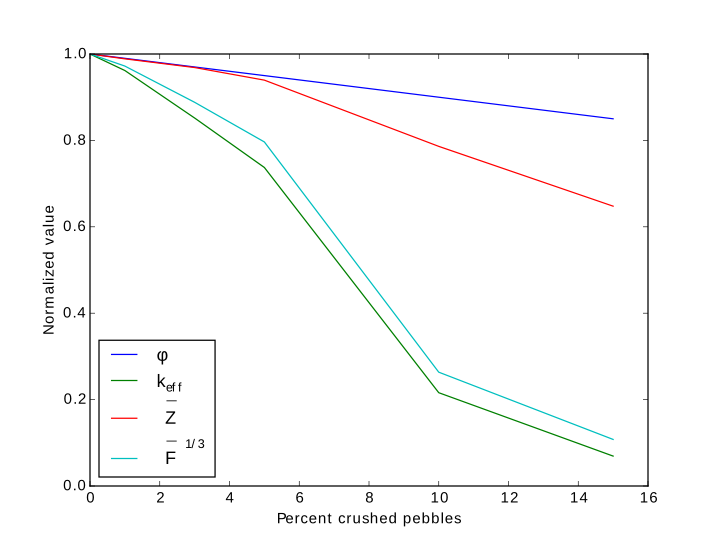
\includegraphics[width=\singleimagewidth]{chapters/figures/kEff_packingFraction}
	\caption{The normalized effective conductivity drops much more rapidly than the normalized packing fraction, $\phi$, while pebbles are crushed. The effective conductivity follows with reduced normal contact forces.}
\label{fig:packing-fraction}
\end{figure}

The large reduction in normal contact force (which leads to a large reduction in effective conductivity) is explainable based on the experimental setup of our numeric model. In our system, we had rigid walls in the $x$ and $z$ directions. These walls did not change after the substantial number of pebbles were crushed and removed. After the 15\% crushing event, the pebble bed appeared as Fig.~\ref{fig:15percent-crushed-pre}. A massive re-arrangement proceeds from the crushing event. As the pebble bed heats up, the thermal expansion of the pebbles is unconstrained as there exists an average of two pebble diameter gap above the pebbles to the top of the container. Numerically there is no limit to the pebble temperatures (phase change and sintering is not incorporated into the DEM calculations) so the pebbles heat and swell until coming into contact with the top wall, at which time they begin to press into one another (though lightly) to allow thermal conduction. The pebble bed after swelling is shown in Fig.~\ref{fig:15percent-crushed-swelling}.

\begin{figure}[!ht]
	\centering
	\begin{subfigure}[t]{\doubleimagewidth}
		\centering
		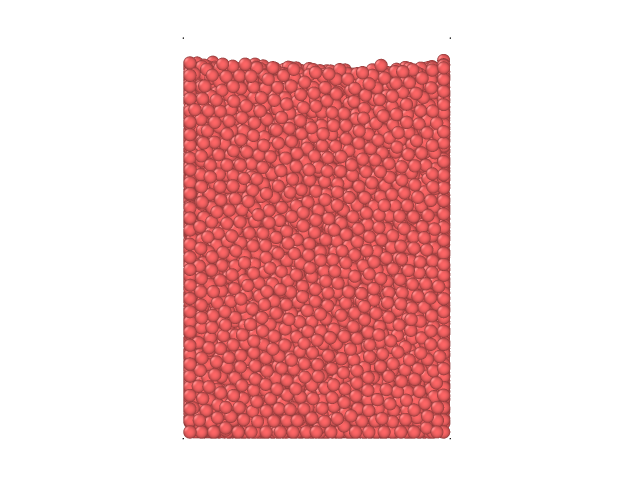
\includegraphics[width=\textwidth]{chapters/figures/heating_dte-02/15/0.15_pre_heat.png}
		\caption{Side-view of the pebble bed after resettling from the crushing event, before heating.}
		\label{fig:15percent-crushed-pre}
	\end{subfigure}
	\begin{subfigure}[t]{\doubleimagewidth}
		\centering
		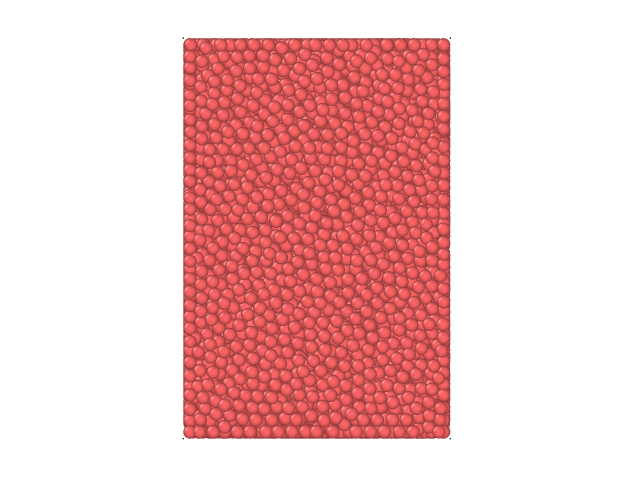
\includegraphics[width=\textwidth]{chapters/figures/heating_dte-02/15/0.15_post_heat.png}
		\caption{Side-view of the pebble bed after heating}
		\label{fig:15percent-crushed-swelling}
	\end{subfigure}
	\caption{In (a) we see the pebble bed after 15\% of the pebbles have been crushed (removed) and then after the heating cycle in (b). The gap formed after crushing is completely filled by swelling pebbles.}
\end{figure}





\FloatBarrier

\subsection{Comparison of Young's Modulii Used in DEM Simulations}\label{sec:dem-studies-youngs-modulus}

The discrete element method is used by many ceramic breeder researchers to model the interaction of individual pebbles in an ensemble.\cite{An20071393, Lu2000, Zhao2010, Gan:2010uq, Annabattula2012a, VanLew2014} In the past studies, the Young's modulus of the ceramic materials used in DEM simulations was taken from historical data, for instance lithium metatitanate from Ref.~\cite{Gierszewski1998}. However, in the previous section I proposed a modification of the Young's modulus to be used in DEM simulations for a batch of ceramic pebbles based on the `softening' seen of most pebbles in experiments. The force-displacement curves of Figs~\ref{fig:fzk-exp-hertz} and~\ref{fig:nfri-exp-hertz} demonstrate how far from the ideal Hertzian curves the majority of of ceramic pebbles behave.

The Hertzian force is linearly proportional to the pair Young's modulus of contacting spheres. Based on the $\kappa$ values found in \cref{sec:exp-reduction-factor}, the apparent Young's modulii of \lis~and \lit~are, on average, less than half the values given for sintered materials in literature. For the case of \lit, the average value was closer to only 10\% of the value from literature. Thus the actual contact forces in pebble beds may be 10\% of the values found from DEM simulations with incorrect Young's modulus! The contact force is a critical value for determining the conduction heat transport between pebbles as well as damage prediction. It is crucial to use proper material properties in our simulations in order to have dependable predictions of pebble crushing events and heat transfer. In this section, I will compare a number of pebble beds under numerical simulations of uniaxial compression tests. One set of beds will be composed of pebbles with the single Young's modulus from literature and the other set will be composed of pebbles with a distribution of Young's modulii that fit the distribution from experiments.
%~~~~~~~~~~~~~~~~~~~~~~~~~~~~~~~~~~~~~~~~~~~~~~~~~~~~~~~~~~~~~~~



%~~~~~~~~~~~~~~~~~~~~~~~~~~~~~~~~~~~~~~~~~~~~~~~~~~~~~~~~~~~~~~~
\subsubsection{Numerical Setup}
%In pebble bed breeder units, the stresses on the pebble regions are a result of thermal expansion of the relatively hot pebbles contained by relatively cool container walls. This process is a function of the coefficient of thermal expansion of the pebbles and their elevated temperature; the confined strain relates to a stress. 
The pebble beds are modeled as undergoing a standard uniaxial compression up to 6 MPa while measuring the macroscopic stress-strain for some parametrically varied pebble beds. At the moment of maximum stress, we can investigate the differences in contact forces of the different pebble beds.

Our pebble ensemble is composed of \SI{0.5}{\milli\meter} diameter \lis~pebbles. The pebble beds are initiated and packed in the same manner as \cref{sec:dem-studies-effective-conductivity} (more details can be found in that section). There are two main bed groups. Set A: three beds (A.1-3) containing a single type of pebble with $E$ = \si{90 GPa}. Set B: four beds (B.1-4) containing ten types of pebbles with their Young's modulus assigned in a discrete, random way to satisfy the distribution seen from experimental data. For the DEM study, I fit the \lis~pebbles with a Weibull distribution of shape parameter $\sigma = 1.6$ where the average stiffness was $\bar{E} = 49$~GPa. The description of the two sets of pebble beds is visually represented in Fig.~\ref{fig:dem-types}. The pebble bed geometry was also the same used in the study of Ref.~\cite{VanLew2014}~: two virtual walls in the x-direction located at $x_\text{lim} = \pm 20 R_p$, periodic boundaries at the limits of $y_\text{lim} = \pm 15 R_p$, and a total of 8000 pebbles packed into the volume to an approximate height of $z_\text{lim} = 20 R_p$.

Among both sets, a parametric study was done on pebble radius and coefficient of friction. The radii of pebbles in beds A.1, A.2, B.1, and B.2 were constant at $R_p$=.25 mm. The radii of pebbles in beds A.3, B.3, and B.4 followed a Gaussian distribution about $\bar{R}_p$ = 0.25 mm: $\mu_d = R_p$ and $\sigma_d = R_p$. The coefficient of friction was set at $\mu = 0.2$ for beds A.1, A.3, B.1, and B.3; the coefficient of friction was $\mu = 0.3$ for beds A.2, B.2, and B.4.


\begin{figure}[t]
  \centering
  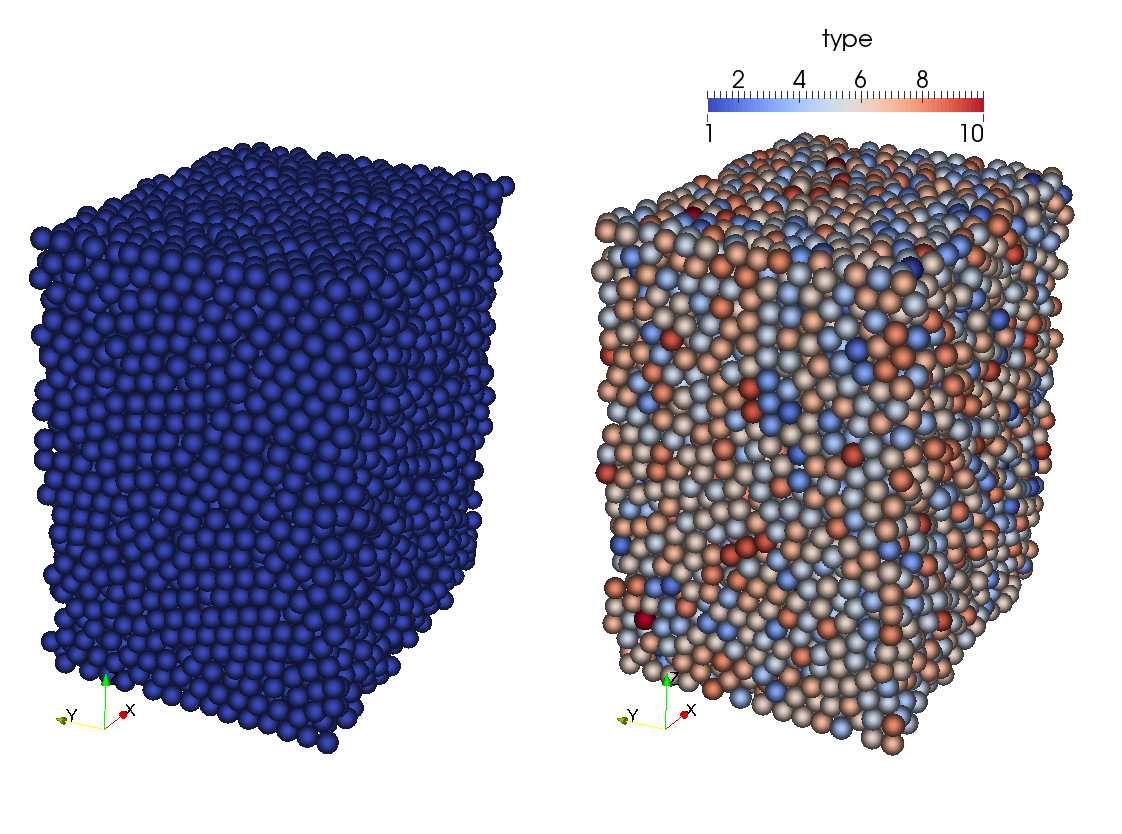
\includegraphics[width=\singleimagewidth]{chapters/figures/DEM-types}
  \caption{On the left, set A, a pebble bed with a single type, of $E = 120$ GPa. On the right, set B, is a pebble bed with 10, randomly distributed types; each type corresponds to a reduced, apparent Young's modulus as derived from experimental data.}\label{fig:dem-types}
\end{figure}
%~~~~~~~~~~~~~~~~~~~~~~~~~~~~~~~~~~~~~~~~~~~~~~~~~~~~~~~~~~~~~~~





%~~~~~~~~~~~~~~~~~~~~~~~~~~~~~~~~~~~~~~~~~~~~~~~~~~~~~~~~~~~~~~~
\subsubsection{Results from Uniaxial Compression}


A constant-velocity, uniaxial compression was applied to the pebble beds. A single cycle up to \SI{6}{\mega\pascal} then down to \SI{0}{\mega\pascal} was used on all the beds. The macroscopic measurements of stress-strain are shown for all the pebble beds in Fig.~\ref{fig:stress-strain}.

\begin{figure}[t]
  \centering
  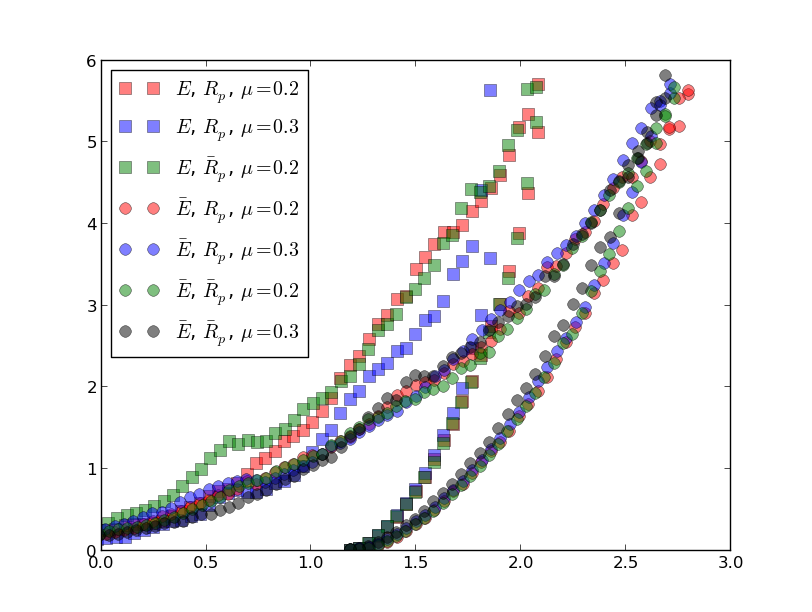
\includegraphics[width=\singleimagewidth]{chapters/figures/stress-strain}
  \caption{Stress-strain responses of pebble beds with: squares, constant Young's modulus; and circles, Gaussian distribution of Young's modulus. The constant Young's modulus beds all had much firmer responses for all parametric cases studied here.}\label{fig:stress-strain}
\end{figure}

Naturally, the pebble beds with smaller Young’s modulus (with circle markers) are more compliant to external loads. The result is true regardless of the coefficient of friction or distribution of pebble radius studied here. Group B moved to an average strain of about 2.6\% at \SI{6}{\mega\pascal}, by comparison the beds of Group A only had strained 1.9\% on average to reach the same stress. Among the beds of each group, pebble beds with constant radius pebbles behaved virtually the same as similar pebble beds with a Gaussian distribution on radius. An increase in the coefficient of friction had a moderate impact on the overall stress-strain response. 


The parametric study here shows that the largest contributor to stress-strain response is the Young’s modulus. The coefficient of friction and radius distribution had comparatively insignificant influence. A pebble bed geometry more directly comparable to oedometric compression experiments should be used to allow direct comparison and validation of the numerical models.


At the point of peak stress for each bed, I use DEM results to visualize the distribution of contact forces among all pebbles in the ensemble. A plot of the probability distributions of all the beds together, Fig.~\ref{fig:all-contact-forces}, shows that the majority of the contacts in all the beds are equally small. There are a few overall trends we observe from the results however. The pebble beds with the constant Young's modulus are always higher for their comparable version with distributed Young's modulus. For pebble beds with comparable Young's modulii and radii, higher coefficients of friction generally have higher peak contact forces. Pebble beds' radius distributions have much less impact on peak contact forces than either coefficient of friction or Young’s modulus. Another method of comparing overall contact force distributions is to consider predictions on pebble cracking which assigns a strength value at random to pebbles in the bed (details are given in \cref{sec:exp-reduction-factor}). At the point of maximum stress, this is done and the results are shown in Table~\ref{tab:num-crush-percent}.

While overall the predicted number of broken pebbles is small, we compare similar parameteric pebble beds and in each case pebble beds with modified Young’s modulus overall predict smaller percentages of broken pebbles. Pebble crushing is a major topic for the overall evaluation of the feasibility of ceramic pebble beds in fusion reactors. This study reveals that past DEM work on pebble crushing, such as Ref.~\cite{Annabattula2012a,Annabattula2014,Zhao2013}, were likely over-predicting the extent of crushing if the Young's modulus used in the study was much larger than the realistic response of individual pebbles.

\begin{figure}[t]
  \centering
  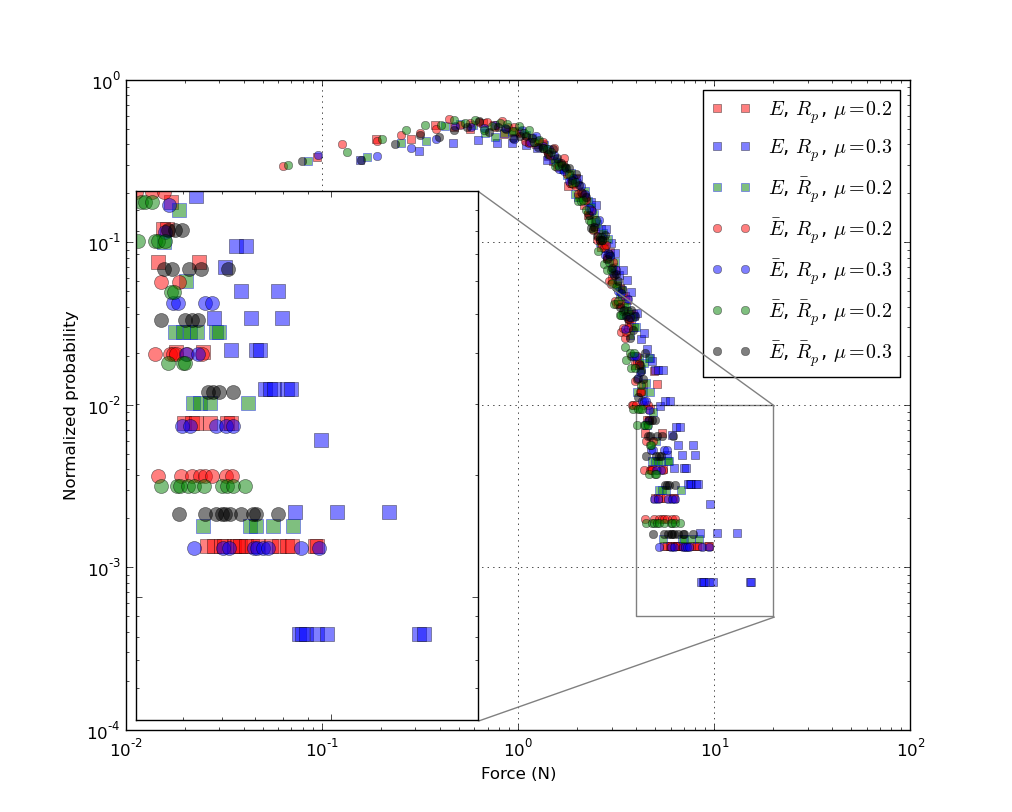
\includegraphics[width=\singleimagewidth]{chapters/figures/all-contact-forces}
  \caption{Probability distribution of contact forces in all the pebble beds studied here. Elastic moduli value is the largest contributor to higher peak contact forces among pebbles.}\label{fig:all-contact-forces}
\end{figure}


\begin{table}[t]
\caption{Comparisons for the two styles of Young's modulii used in the study. }
\label{tab:num-crush-percent}\centering
\begin{tabular}{llS[table-format=3.2]}
\toprule
Bed label		& 		Parameters 								&	\text{Predicted crushed}			\\
				& 												&	\multicolumn{1}{r}{\text{\%}}		\\\otoprule
A.1				& 		$E$, $R_p$, $\mu = 0.2$          		&	0.3									\\\midrule
A.2				& 		$E$, $R_p$, $\mu = 0.3$     			&	1.0									\\\midrule
A.3				& 		$E$, $\bar{R}_p$, $\mu = 0.2$			&	0.9									\\\midrule
B.1				& 		$\bar{E}$, $R_p$, $\mu = 0.2$			&	0.6									\\\midrule
B.2				& 		$\bar{E}$, $R_p$, $\mu = 0.3$			&	0.8									\\\midrule
B.3				& 		$\bar{E}$, $\bar{R}_p$, $\mu = 0.2$		&	0.4									\\\midrule
B.4				& 		$\bar{E}$, $\bar{R}_p$, $\mu = 0.3$		&	0.7									\\\bottomrule
\end{tabular}
\end{table}
%~~~~~~~~~~~~~~~~~~~~~~~~~~~~~~~~~~~~~~~~~~~~~~~~~~~~~~~~~~~~~~~






%~~~~~~~~~~~~~~~~~~~~~~~~~~~~~~~~~~~~~~~~~~~~~~~~~~~~~~~~~~~~~~~
\subsection{Conclusions of Young's Modulus Study}
Variation in production techniques for ceramic pebbles have lead to batches of pebbles with slight differences in their ceramic microstructure, as evident in the wide distribution of crush loads reported in past studies, \textit{e.g.} Refs.~\cite{Zhao2012,Mandal2012a}. By the same token, the different microstructures should naturally lead to variation in Young’s modulus. However up to now values of Young’s modulus used in numerical models are taken from values measured for large sintered pellets of ceramic materials. Based on single pebble experiments and the application of Hertz theory, a technique for introducing a modified Young’s modulus into DEM models has been proposed here. DEM simulations show the impact of modified pebble elasticity on both macroscopic measurements of stress-strain curves as well as mesoscopic measures of inter-pebble contact force -- with major implications for prediction of pebble crushing in ceramic pebble beds and macroscopic $\sigma-\epsilon$ responses. The models applying the softening coefficient, $\kappa$, predict more compliant pebble beds and smaller peak contact forces in beds and thus fewer crushed pebbles.

Thus I conclude that in DEM numerical models for pebble damage, the modified Young's modulus with softening coefficients matching the probability density function from experiments must be used. In this way, we can expect a more realistic numerical tool to simulate pebble damage, bed rearrangement, and heat transfer.
\section{Stability study}\label{sec:dem-stability}
As mentioned when the integration algorithm was introduced in \cref{sec:particle-dynamics}, the velocity-Verlet algorithm is a computationally efficient, second-order accurate means of updating the kinematics of all the particles in the ensemble\cite{Kruggel-Emden2008}. The timestep of the integration, however, must often be very small to ensure that it is less than the time taken for a pressure wave to propagate through the particle. The timestep is further constrained by the quasistatic assumption used to derive the Hertzian contact force such that inertial and relaxation effects may be neglected\cite{Brilliantov1996}. We will also show that, in order to avoid heat energy to propagate further than a single pebble during a single timestep, the thermal timestep requirement is orders of magnitude larger than the mechanical timestep equivalent. And that the overall minimum timestep is thus driven by the mechanical stability.

In tandem with the requirement on very small timestep, the thermal time-constants in the ceramic breeder zones can be many hundreds of seconds. These two conditions seem to conspire to force an unacceptably large requirement on the number of timesteps for a thermal DEM simulation and thus make numerical experiments impractical.

In this section we will analyze the calculation of a critical timestep based on the speed of a Rayleigh wave propagating along the surface of a particle. Then, with that knowledge in hand, we will argue for scaling certain physical properties to allow for faster simulations without sacrificing fidelity to the real physics of the problem.


%~~~~~~~~~~~~~~~~~~~~~~~~~~~~~~~~~~~~~~~~~~~~~~~~~~~~~~~~~~~~~~~~~~~~~~~~~~~~~~~~
\subsection{Critical dynamic timestep}
If we wish to choose a timestep sufficiently small such that a pressure wave originating from the contact of one particle does not propagate to other neighboring particles during the timestep, we must choose a timestep smaller than the critical timestep defined by Rayleigh wave traveling through the solid.

When a force is applied to the surface of an elastic body, the force propagates along the surface at the wave speed first solved by John William Strutt, 3rd Baron Rayleigh\cite{Rayleigh1885} (when he wasn't discovering the scattering phenomenon explaining why the sky is blue or winning the Nobel prize for discovering Argon),

\begin{equation}
	u_{\Ra} = K\sqrt{\frac{G}{\rho}}
\end{equation}

where, again, $G$ is the shear modulus and $\rho$ is the density of the elastic material. The $K$ coefficient is a complicated function coming from Rayleigh's solution but can be approximated as\cite{Sheng2004}

\begin{equation}
	K = 0.1631 \nu + 0.876605
\end{equation}

which is valid for realistic values of Poisson's ratio, $\nu$, of elastic materials. From the inverse of the Rayleigh wave frequency, we can directly find a timestep for Rayleigh waves on a sphere of radius, $R$,

\begin{equation}\label{eq:rayleigh-stability-time}
	\delta t_{\Ra} = \frac{\pi R}{u_{\Ra}}
\end{equation}

When we write this for any particle, $i$ in the ensemble (exchanging the shear for elastic modulus),

\begin{equation}\label{eq:rayleigh-timestep}
	(\delta t_{\Ra})_i = \frac{\pi R_i }{0.1631 \nu_i + 0.876605} \sqrt{\frac{2(1+\nu_i)\rho_i}{E_i}}
\end{equation}

We allow for the particles in the system to have varying density, elastic modulus, and size. Therefore the critical timestep for the entire system is governed by the minimum value of any particle's Rayleigh timestep. 

\begin{equation}
	\delta t_c = \min_{\forall i}\left[(\delta t_{\Ra})_i\right]
\end{equation}


% \begin{align}
% \delta t_c = \eta  \sqrt{\frac{m_0}{k_0}}
% \end{align}
% where $m_0$ is the smallest particle mass, related to the smallest particle radius, $R_0$. The value of $\eta$ is less than unity and depends on the integration algorithm as well as dimensions of freedom [site O'Sullivan].
% \begin{align}
% m_0 = \frac{4}{3} \pi R_0^3 \rho
% \end{align}
% and we assume all pebbles have the same density, $\rho$. $k_0$ is the maximum normal stiffness in the ensemble. The timestep chosen for the DEM must be less than this critical timestep.
% \begin{align}
% \Delta t \le \delta t_c
% \end{align}

% From Hertz theory, the maximum normal contact stiffness is
% \begin{align}
% k_0 = \frac{4}{3} E^* \sqrt{R^*_0 \delta_0}
% \end{align}

% To find the maximum contact stiffness (neglecting the influence of $\delta_0$ for the moment), we will express the relative radius in an alternate form,
% \begin{align}
% \frac{1}{R^*_0} = \frac{1}{R_0} + \frac{1}{\gamma R_0}
% \end{align}
% where $\gamma \ge 1$, it is a parameter that indicates our smallest pebble of radius $R_0$ is interacting with another pebble that is either the same size or larger. In the limits, if $\gamma =1$, then $R^*_0 = \frac{R_0}{2}$. If $\gamma \rightarrow \infty$, then $R^*_0 = R_0$. The stiffness is positively proportional to relative radius. Therefore if we desire the maximum contact stiffness, we need the largest value of $R^*_0$ and thus require $\gamma \rightarrow \infty$.

% With $R^*_0 = R_0$, we use this in the formula for pebble mass term of the stability criteria 
% \begin{align}
% \delta t_c &= \eta  \sqrt{\frac{\frac{4}{3} \pi (R^*_0)^3 \rho}{\frac{4}{3} E^* \sqrt{R^*_0 \delta_0}}}\\
% \delta t_c &= \left[ \eta \sqrt{ \pi} \right] \rho^{1/2}\left(\frac{1}{E^*}\right)^{1/2} \left(\frac{1}{\delta_0}\right)^{1/4}(R^*_0)^{5/4}
% \end{align}

% We can relate the maximum pebble overlap $\delta_0$ to the maximum contact force in the ensemble with Eq.~\ref{eq:hertzForce}, after some algebra we find
% \begin{align}
% \delta t_c &= \left[ \eta \sqrt{ \pi} (4/3)^{1/6} \right] \rho^{1/2} \left(\frac{1}{F_\text{max}}\right)^{1/6} \left(\frac{1}{E^*}\right)^{1/3} R^{*5/4}_0
% \end{align}

% The term in the bracket is a constant near unity. Neglecting it, we see the timestep is proportional to these terms,
% \begin{align}\label{eq:stability-terms}
% \delta t_c \propto \rho^{1/2} \left(\frac{1}{F_\text{max}}\right)^{1/6} \left(\frac{1}{E^*}\right)^{1/3} R^{*5/4}_0
% \end{align}

% Figure~\ref{fig:stability-curves} provides visual reinforcement of the powers of terms in Eq.~\ref{eq:stability-terms}; it is the impact of different normal-contact parameters on the stable timestep. 
% \begin{figure}[ht!]
% \centering
% 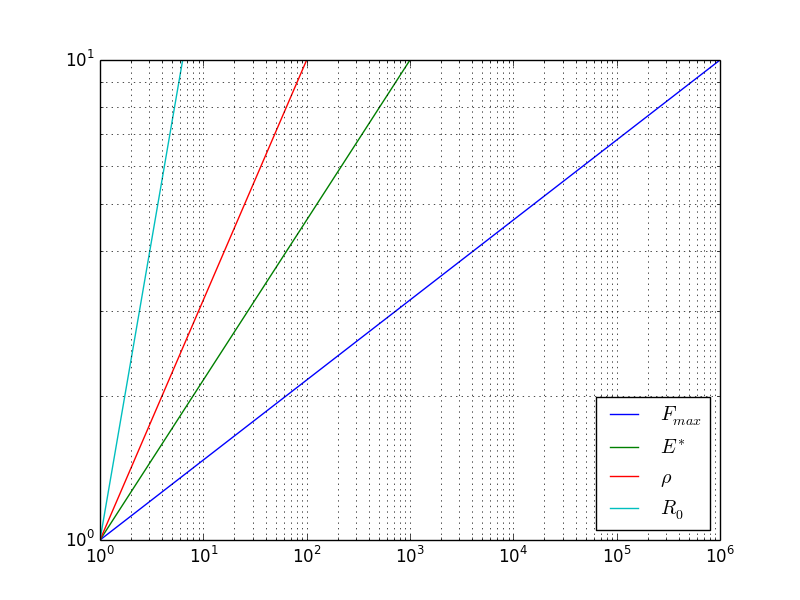
\includegraphics[width = 0.75 \textwidth]{chapters/figures/stability_curves}
% \caption{Curves showing the rate of response to timestep on the various normal-contact parameters.}\label{fig:stability-curves}
% \end{figure}

% It is apparent that simulations become less stable primarily as the pebble diameter decreases and then slightly less so for decreasing density and increasing the effective Young's modulus. It takes a rather large increase in the maximum contact force to cause the stable timestep to decrease. This is a fortunate result as it is primarily material properties which dictate stability of a DEM simulation. If external pressures increase and cause increases in the maximum normal contact force in the ensemble, it is unlikely to cause instabilities in the model. The result also provides insight into scaling of physical parameters to allow larger timesteps and thereby shorter overall duration of simulations.

The ceramic materials identified for breeders have relatively high Young's moduli, on the order of \si{10^{10} Pa}. The smallest radius will be on the order of \si{10^{-4} m}. The ceramic density is approximately on the scale of \si{10^{4} kg/m^3}. These values lead to a necessary timestep of

\begin{equation}
	\delta t_c \propto 10^{-7} \si{s}
\end{equation}

For a simulation that may last several hundreds of seconds of real time, this then requires more than 10$^9$ timesteps. If we have 10$^4$ particles in the simulation, each having their position integrated over a billion times, it becomes obvious that computational time is a major issue for our simulations of nuclear heating of ceramic breeder pebbles. If we are able to reduce the critical timestep (while perhaps decreasing the simulation time), the simulations will be much more practical for research use.
%~~~~~~~~~~~~~~~~~~~~~~~~~~~~~~~~~~~~~~~~~~~~~~~~~~~~~~~~~~~~~~~~~~~~~~~~~~~~~~~~




%~~~~~~~~~~~~~~~~~~~~~~~~~~~~~~~~~~~~~~~~~~~~~~~~~~~~~~~~~~~~~~~~~~~~~~~~~~~~~~~~
\subsection{Critical thermal timestep}

In \cref{sec:ht-pebble-conduction}, we introduced the dynamics of heat transfer between contacting particles in an ensemble. As we integrate the energy of an individual particle in time, we must also ensure that energy would not propagate through a particle faster than a single timestep can capture. In analogy to the critical timestep for mechanical stability (e.g. Eq.\ref{eq:rayleigh-stability-time}), we write for particle $i$,

\begin{equation}
	\delta t_\Bi = \frac{\rho_i C_i V_i}{H_c}
\end{equation}

where $\rho_i C_i V_i$ represents the inertial resistance to changing the temperature of $T_i$ and the conductance, $H_c$ represents the speed at which energy is delivered to $T_i$ from contact conduction. Then from the definition of $H_c$ we have given for smooth elastic spheres, this is also written as

\begin{equation}
	\delta t_\Bi = \frac{(4/3)\pi R_i^2\rho_i C_i}{2k^*}\frac{R_i}{a}
\end{equation}

For the material properties of lithium ceramics, as discussed for mechanical stability, we can expect

\begin{equation*}
	\frac{(4/3)\pi R_i^2\rho_i C_i}{2k^*} \approx \frac{(10^{-4})^210^{4}10^3}{10^0} = 10^{-1}
\end{equation*}

But from the requirements on Hertz theory in \cref{sec:hertz-theory}, we have required that $\frac{a}{R_i} \ll 1$. Thus the timestep for stability in the energy calculation is utterly negligible compared to the mechanical stability.

Vargas and McCarthy\cite{Vargas2001} make similar arguments, giving the criteria as,

\begin{equation}
	\frac{\mathrm{d}T_i}{T_i - T_j} \ll 1
\end{equation}

and too note that the timestep requirement for thermal calculations are orders of magnitude less restrictive than the analogous restriction of the particle dynamics.

Thus we can be confident that any timestep chosen for dynamic stability in the DEM simulation will automatically satisfy the timestep for thermal stability. 
%~~~~~~~~~~~~~~~~~~~~~~~~~~~~~~~~~~~~~~~~~~~~~~~~~~~~~~~~~~~~~~~~~~~~~~~~~~~~~~~~





%~~~~~~~~~~~~~~~~~~~~~~~~~~~~~~~~~~~~~~~~~~~~~~~~~~~~~~~~~~~~~~~~~~~~~~~~~~~~~~~~
\subsection{Simulation acceleration with scaled material properties}

We rewrite Eq.~\ref{eq:rayleigh-timestep} to facilitate a discussion on the parameters. Isolating each material term (neglecting the Poisson ratio) gives, 

\begin{equation}
	\delta t_c \propto R_i \times \rho_i^{1/2} \times E_i^{-1/2}
\end{equation}

% [pretty sure the approximation for $\nu$ only works when it's less than 1 so can't scale. must find out for sure.]

% The most direct effect would come from scaling the radius 





% From Makse\cite{Makse2004}

% We choose the time step to be a fraction of the time that it takes for a sound wave to propagate on the grain. Moreover, the quasistatic approximation used to calculate the Hertz force is valid only when the relative velocities of the par- ticles is smaller than the speed of sound in the grains\cite{Brilliantov1996}. Thus the characteristic time is $t_0 = R\sqrt{\rho_r/\mu_r}$ Typically, one chooses a time interval much smaller than the characteristic time, then $\Delta t=aR \sqrt{\rho_r/\mu_r}$ with $a<1$. Typical values for glass beads are:
% \si{\rho =2600 kg/m^3}, \si{\mu_r = 29 GPa}, \si{R = 0.1 mm}. Then $\Delta t$ should be smaller than \si{10^{−8} s}. Thus in order to perform a simulation over one second, more than $10^8$ steps are needed, which is obviously a very intensive computation. In this case, it is customary to increase the density or decrease the rigidity of the particles to allow for a larger time step to integrate the equations of motion over realistic periods of time. If the shear modulus of the grains in decreased, then it should be checked that the resulting stresses are several order of magnitude smaller than $\mu_r$, thus ensuring the condition of a nearly rigid system even though $\mu_r$ is taken smaller to obtain larger timesteps.
\subsection{Conclusions}
\label{sec:dem-conclusions}
The results shown in Figs.~\ref{fig:contact-forces-scatter} and~\ref{fig:coord-scatter} demonstrate that the heat transfer through a pebble bed is simultaneously a function of both the coordination number and inter-particle contact forces. The average values of both of these parameters reduced as pebbles in the bed were crushed. Interestingly, when a pebble bed has lower overall inter-particle contact forces such as what we see when pebbles are crushed, we would predict fewer pebbles are likely to break. This result implies that pebble breakage is self-dampening; as pebbles begin to break the ensemble quickly relaxes and avoids future pebble failure. So while in this study we induced failure up to $\eta = 15\%$ without a concern for predicting if such a large amount would break, such large values may not occur in real beds during operation of a fusion reactor. 

The first study of this dissertation established the groundwork of the DEM modeling to be carried out in the other studies. We simulated a pebble bed with a specified fraction of the pebbles crushing during operation; then determining the repercussions of the missing pebbles as they affect the macroscopic property of effective thermal conductivity. We used the assumption of homogeneous, random locations of pebble failure to induce a failure routine without requiring external loads on the bed to actually induce the pebble crushing. After heating to a steady-state, an effective thermal conductivity was calculated for the pebble bed. The results show that large amounts of pebble failure correspond to large decreases in the conductive transport of energy through the pebble bed. The increase was due primarily to a drop in the inter-particle forces which lead to a large increase in temperature differences between neighboring pebbles. 

As the first step in the modeling effort, there were many simplifications that had to be made in this study. We must note here the shortcomings of the assumptions and simplifications of this study before drawing any major conclusions from the results.

First, the `container walls' surrounding the pebble bed in this model are completely rigid and do not react as the swelling pebble bed presses into them while heating. The confined thermal expansion leads to very high contact forces in the pebble bed that may not be realistic. The abnormally high contact forces are most likely to be the source of the abnormally high baseline effective thermal conductivity, $k_0 = 1.03$~W/m-K. In experiments on the effective thermal conductivity of lithium ceramics in vacuum, the beds are often allowed to expand freely while heating (in at least one direction) and in vacuum were measured to be closer to $k_0 = 0.2$ W/m-K.[cite ali abou sena] We note, however, that this value has been calculated in the absence of interstitial gas so the results apply only to the reduction in energy transferred via inter-particle conduction.

Second, we saw from Fig.\ref{fig:temp-scatters} that the majority of the pebbles in the ensemble have their temperatures close fitting to an average curve but a number of the pebbles had less thermal contact with neighboring particles and consequently had much larger temperatures. This was true even in the baseline case of a tightly packed ($\phi = 64\%$) pebble bed. This phenomena is only possible because the contribution to heat transfer of the interstitial gas was not considered in this model. The flowing helium gas is expected to prevent any runaway temperatures of individual pebbles as it provides another route of energy transfer in the bed. This will be addressed in \cref{sec:cfd-dem-studies}.

Lastly, the pebble crushing did not conserve mass and did not have predictive whatever.